\documentclass{article}
\usepackage[UTF8]{ctex}
\usepackage{geometry}
\usepackage{natbib}
\geometry{left=3.18cm,right=3.18cm,top=2.54cm,bottom=2.54cm}
\usepackage{graphicx}
\pagestyle{plain}	
\usepackage{setspace}
\usepackage{caption2}
\usepackage{datetime} %日期
% \usepackage{url}
\usepackage[colorlinks,linkcolor=black]{hyperref}
\renewcommand{\today}{\number\year 年 \number\month 月 \number\day 日}
\renewcommand{\captionlabelfont}{\small}
\renewcommand{\captionfont}{\small}
\begin{document}

\begin{figure}
    \centering
    
\includegraphics[width=8cm]{upc.png}

    \label{figupc}
\end{figure}

	\begin{center}
		\quad \\
		\quad \\
		\heiti \fontsize{45}{17} \quad \quad \quad 
		\vskip 1.5cm
		\heiti \zihao{2} 《计算科学导论》课程总结报告
	\end{center}
	\vskip 2.0cm
		
	\begin{quotation}
% 	\begin{center}
		\doublespacing
		
        \zihao{4}\par\setlength\parindent{7em}
		\quad 

		学生姓名:\underline{\qquad  田康康 \qquad \qquad}

		学\hspace{0.61cm} 号:\underline{\qquad 1606050112\qquad}
		
		专业班级:\underline{\qquad 计科1702 \qquad  }
		
        学\hspace{0.61cm} 院:\underline{计算机科学与技术学院}
% 	\end{center}
		\vskip 2cm
		\centering
		\begin{table}[h]
            \centering 
            \zihao{4}
            \begin{tabular}{|c|c|c|c|c|c|c|}
            % 这里的rl 与表格对应可以看到,姓名是r,右对齐的;学号是l,左对齐的;若想居中,使用c关键字。
                \hline
                课程认识 & 问题思 考 & 格式规范  & IT工具  & Latex附加  & 总分 & 评阅教师 \\
                30\% & 30\% & 20\% & 20\% & 10\% &  &  \\
                \hline
                 & & & & & &\\
                & & & & & &\\
                \hline
            \end{tabular}
        \end{table}
		\vskip 2cm
		\today
	\end{quotation}

\thispagestyle{empty}
\newpage
\setcounter{page}{1}
% 在这之前是封面,在这之后是正文
\section{引言}
计算科学导论\citep{book1}本来应该初入大学的时候学习,但是因为我是半路出家,大二才从储建院转专业至计通院,而且因为选课原因没有在转过来的当年选修上当时的计算机科学导论,所以只得推迟到大三的上学期来学习这门课程。虽然已经大三了,对未来的学习或是工作已经有了大致的规划,但是通过学习导论,还是收获了很多原来没有考虑过或者说涉足过的知识与观念。\par

\section{对计算科学导论这门课程的认识、体会}
“计算科学导论”,顾名思义,是一个对计算机专业的概括性、引导性的课程。导论也称作引论,
是论著正文前概要论述全文或全书的中心思想、创作思路、背景和创作方向的简单概括叙述,以指导帮助读者阅读理解的部分。
关于学科的导论是指用较为概括的语言来论述这一学科的基本的和整体的思想,从而使读者对该学科有较为整体和系统的把握。\par
在上这门课之前,我觉得自己对计算机专业的大致了解还是可以的,除了对自己感兴趣的前端、Python等略有深入外,对现在主流的技术、框架都有所了解,但是却没有更深入的思考。
直到学习了“计算科学导论”后,我才意识到计算机专业不止有“计算机科学与技术”,还有更深层次的“哲学”需要我们去探索。这已经不是技术层面的理解了,是从思想层面的层层深入。\par


\subsection{科学哲学的思想方法}
本章的开头提到了一句话——真正理解一件事物最好的方式莫过于去探寻它的历史——我觉得很有道理。
当一件事物、一个学科发展几年、几十年甚至几百年时,大多数人对这个已经略显成熟的甚至已经止于至善的事物的认识可能只有它所有最新的理论,最通俗的认知。
但是如果想深入地认识这个事物,单纯的从艰深的理论,最新的成果去深入研究是效率低下的。最好的方法其实是追本溯源,追溯到这个理论的源头,认识到它是为什么被提出来的,又是作为什么被研究的。
理解了根源之后,沿着该事物的发展路线,逐步学习、消化它所积淀的知识,才能完全的掌握理论,为己所用。\par

在本学期之前,这门课一直名为“计算机科学导论”,直到本学期才更名为“计算科学导论”,初始选课的时候我对这次改名称有所疑惑,并没有意识到这其中更深层次的原因。当然,我没有听过“计算机科学导论”的上课内容,
我只知道当时结课的任务是提交一份自己的工程代码并且参加闭卷考试,这更像是一个考核性的课程,并没有涉及到理论的上升。但是这一学期的“计算科学导论”上完之后,我觉得收获的并不是可以用考试考核来验证的知识,
更多的是一种思想,一种对计算科学、哲学的认知。\par

“计算科学”一词的来历可以追溯到20世纪30年代到60年代初,当时的工作主要是围绕“什么是计算”开展理论探索,数学问题主要还是靠科学家、数学家手工进行运算。直到图灵机的出现,才有了自动装置计算的开始,
后来有冯•诺依曼等人的贡献,1946年制造出了世界第一台大型计算机“ENAIC”。有了计算机强劲算力的支撑与高级程序设计语言的发展,计算数学的发展突飞猛进,同时多个领域的融合分化催生了计算机科学作为一个学科的出现。
经过发展,计算机科学又分化出了计算机科学与计算机工程两大阵营,各有侧重点,通俗来讲即一个偏软件,一个偏硬件。分化的两大阵营也引起了很多争议与辩论,为了解决分歧,探索一个科学的发展方向,选择了“计算作为一门学科”
这个方向,计算学科囊括了计算机工程、信息技术、信息系统等18个主领域。所以“计算科学导论”其实是“计算机科学导论”的一个超集,概括性更强,有更深厚的历史积淀。\par

科学哲学\citep{curd1998philosophy}是20世纪兴起的一个哲学分支,关注科学的基础、方法和含义,主要研究科学的本性、科学理论的结构、科学解释、科学检验、科学观察与理论的关系、科学理论的选择等。该学科的中心问题是:
什么有资格作为科学,科学理论的可靠性,和科学的终极目的。此学科有时与形而上学、本体论和认识论重叠,例如当它探索科学与真理之间的关系时。\par

有许多关于科学哲学的核心问题,包括科学能否揭示不可观察之事物的真相,甚至科学推理是否可以被证明为合理的,哲学家们没有达成共识。除了这些关于科学作为一个整体的一般性问题,
科学哲学家也思考适用于特定学科例如生物学和物理学的问题。一些科学哲学家还使用当代的科学结果来达到哲学本身的结论。\par

但是我们要意识到:我们应该相信科学,迄今为止科学方法是我们能够发现具有真理性知识的最高方法,但是我们也不能迷信科学、迷信科学家,我们要有自己的判断力。
在面对科学结论时,我们需要自己审视它本身的科学性问题,这就是对我们的科学素养、科学常识的考验了。

% 图片插入的样例:\par
% \begin{figure}[h!]
% \centering
% \includegraphics[scale=1.7]{universe}
% \caption{The Universe}
% \label{fig:universe}
% \end{figure}

\subsection{计算机科学的基本概念和基本知识}
% 表格插入样例:\par
% \begin{table}[h]
%     \centering
%     \caption{这是科学系的花名册}
% \begin{tabular}{rl}
% % 这里的rl 与表格对应可以看到,姓名是r,右对齐的;学号是l,左对齐的;若想居中,使用c关键字。
%     \hline
%     姓名 & 学号 \\
%     \hline
%     张三 & 190704xxxx+++ \\ 
%     李四 & 190704yyyy \\
%     王二五 & 190704zzzz\\
%     \hline
% \end{tabular}
%     \label{table1}
% \end{table}
本章是对计算机科学、计算机组成原理、计算机主要研究方向等的概括介绍。作为大三学生,这其中提到的绝大部分内容我都已经系统的学习过。
本章中不止介绍了学科基础方向,也对现在、未来的热门领域进行了展望,其中我最感兴趣的是人工智能与机器学习领域。\par
我现在正在参与“基于暗通道先验的图像去雾”大创项目,
本来我们的技术栈只使用了opencv、numpy等基础库,但是经过几个版本的迭代后发现使用卷积神经网络的单张图像去雾AOD-Net\citep{aod}算法效果更好,而且实现简单。我们最初使用的去雾算法
是基于物理模型的复原方法,这种方法通过研究大气悬浮颗粒对光的散射作用, 建立大气散射模型,了解图像退化的物理机理, 并复原出未降质前的图像。现在对暗通道先验的图像去雾的研究都是基于
何凯明博士的《Single image haze removal using dark channel prior》\citep{dehaze}。这种算法的原理是在绝大多数非天空的局部区域里,某一些像素总会有至少一个颜色通道有很低的值。
换言之,该区域光强度的最小值是个很小的数,这就是暗通道。\par
我们给暗通道一个数学定义,对于任意的输入图像J,其暗通道可以用下式表达:
\begin{equation}
J^{dark}\left ( x \right )=\min_{c\in\left \{ r,g,b \right \}\;\;y\in\Omega \left ( x \right )}\left ( min(J^{c}(y)) \right )
\end{equation}\par
众所周知,雾天中的拍摄的图片,在雾度比较高的地方成像效果较差,颜色较暗,这就是该算法需要识别并处理的区域。
知道了什么是暗通道之后,还需要雾图形成模型:
\begin{equation}
    I\left ( x \right )=J\left ( x \right )t\left ( x \right )+A\left ( 1-t\left ( x \right ) \right )    
\end{equation}\par
$J\left ( x \right )$即是我们需要求得的目标图像。经过一些数学变换后即可得变换公式,这里就不赘述:
\begin{equation}
    J\left ( x \right )=\frac{I\left ( x \right )-A}{max(t\left ( x \right ),t_{0})}+A
\end{equation}\par
这种算法有一个很大的缺点,该算法和以前的技术都是采用构建物理模型与各种复杂的图像统计假设来对图像进行去雾,比如“颜色衰减”模型,场景深度的线性模型,非局部先验的算法等,
而这对于单幅图像来说并没有包含这么多的准确信息,都是通过各种假设来获取到的相关参数,极不准确,所以去雾效果很难令人满意。
所以我们选择了其他的方向,我们的预期便是从单幅图像中直接构建出足够准确的传输矩阵,随着近年卷积神经网络的火热,
我们尝试性地构建了一种可训练的模型来估计一个有雾图像的传输矩阵,使用NYU等经典数据集生成大量的有雾、无雾的对比图对模型进行训练,然后再通过深度学习进行细分,获取足够清晰的去雾图像。\par
经过改进后的算法非常简单,使用了五层卷积神经网络,而且经过大数据集训练而得的模型通用性极佳,对单张图像去雾效果很好。\par
\begin{figure}[ht]
\centering
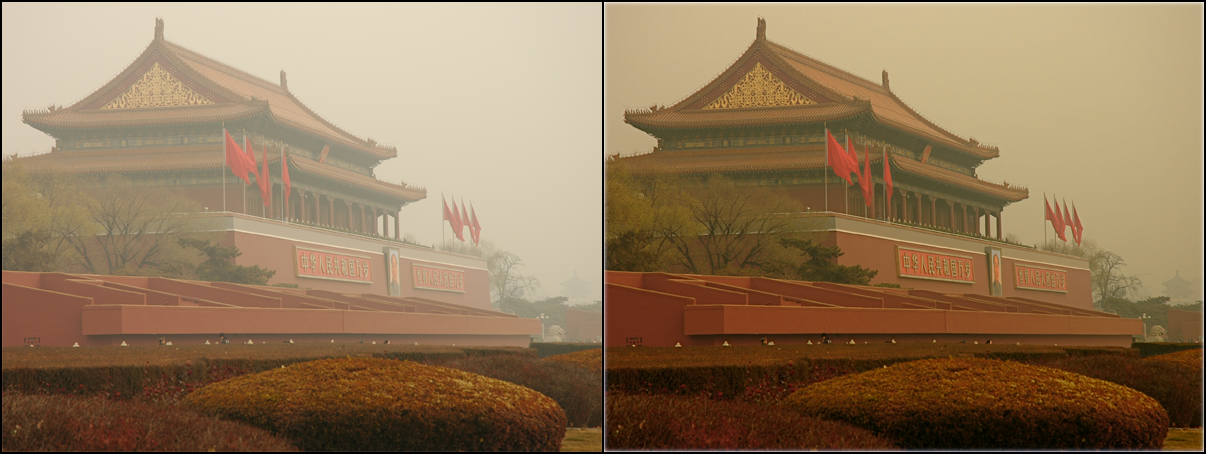
\includegraphics[scale=0.3]{dehaze1.png}
\caption{经典的天安门图像去雾对比}
\label{fig:label}
\end{figure}
亲身体验过机器学习相对于传统算法的优越性之后,我确实被它给“圈粉”了,虽然并不想以后单纯的从事这方面的工作研究,但还是希望在闲暇时可以做一些简单的自己感兴趣的机器学习项目,
比如自动电影推荐系统、音乐推荐系统,提升一下生活体验。

\subsection{计算科学的意义、内容和方法}
什么是计算科学?计算科学是对描述和变换信息的算法过程,包括其理论、分析、设计、效率分析、实现和应用的系统研究。与第一章一样,这里主要要区分的就是“计算科学”与“计算机科学”,虽然只差了一个字,但是所代表的意义大有不同。\par
计算科学的问题域包括数值模拟、模型拟合与数据分析计算优化等领域。同时计算科学中的算法和数学方法也是多样的,
程序设计语言普遍应用于科学计算应用中偏向数学的方面,包括R语言、MATLAB、Mathematica、Scilab、COMSOL Multiphysics、SciPy的Python语言等。偏向于密集型计算的科学计算常会利用C语言或Fortran的一些变体以及BLAS或LAPACK等最优化代数库。
计算科学应用程序常常建立真实世界变化情况的模型,包括天气、飞机周围的气流、事故中的汽车车身变形、星系中恒星的运动、爆炸装置等。这类程序会在计算机内存中建立一个“逻辑网格”,网格中的每一项在空间上都对应一个区域,
并包含与模型相关的那一空间的信息。例如在天气模型中,每一项都可以是一平方千米,并包含了地面海拔、当前风向、温度、压力等。程序会在模拟时步中基于当前状态计算出可能的下一状态,解出描述系统运转方式的方程,然後重复上述过程计算出下一状态。
“计算科学家”一词常用于描述科学计算领域中的技能高超者。他们通常是科学家、统计学家或应用数学家,会以不同方式应用高性能计算机,以提高他们各自的应用学科(如物理学、化学或工程学的相关学科)中最先进的理论和技术水平。科学计算也对经济学、生物学及医学等领域有着越来越大的影响。
计算科学常被认为是科学的第三种方法,是实验/观察和理论这两种方法的补充和扩展。计算科学的本质是数值算法以及计算数学。在发展科学计算算法、程序设计语言的有效实现以及计算结果确认上,人们已经做出了实质性的努力。计算科学中的一系列问题和解决方法都可以在相关文献中找到。\citep{zxx}\par
计算科学自出现至今已经迭代多次,推动计算科学发展的主要动力便是社会广泛的应用需求。从目前来看,计算模型与体系结构、软件开发方法学与计算机应用技术是本学科未来发展的主要方向,而计算理论、体系结构、高等逻辑与形式语义学是支撑学科未来主要方向发展的四大核心专业知识基础。\par
计算科学的意义并没有在内容中出现,我自己进行了总结:计算科学为人类认知世界提供了一种可能的有前途的方法,自出现至今已经引起了人类世界观自然观的巨大变革。而计算机科学和信息科学的极大成就促进了计算概念的普遍化,计算科学为意识提供了一种主流的解释方法,为人工智能技术的发展提供了理论支撑,为理解生命以及基因技术的发展和基于生命科学的计算机技术等提供了理论纲领,有非凡的意义。\par


% {\bf 注意,仅仅是引用的样例}\par
\section{进一步的思考}
在课程中的分组演讲中,我介绍的是“Node.Js”,我觉得有一点与老师的观点有很大分歧——Node的定位适用于前端还是服务端?基于这个分歧点,我又详细的找了一些对Node的介绍,因为这个问题是Node诞生的根本问题,我觉得很有必要搞清楚它到底是什么。\par
首先,我参考了维基百科关于Node的内容。开题即写到“Node.js 是能夠在伺服器端運行 JavaScript 的開放原始碼、跨平台 JavaScript 執行環境”,“在Node.js出現之前,JavaScript通常作為用戶端程式設計語言使用,以JavaScript寫出的程式常在用戶的瀏覽器上執行。Node.js的出現使JavaScript也能用於伺服器端編程。Node.js含有一系列內置模組,使得程式可以脫離Apache HTTP Server或IIS,作為獨立伺服器執行。”。
当然,这是百科上的内容,我们还可以从Node的源码上分析这一问题,下图是Node的源码结构:
\begin{figure}[ht]
\centering
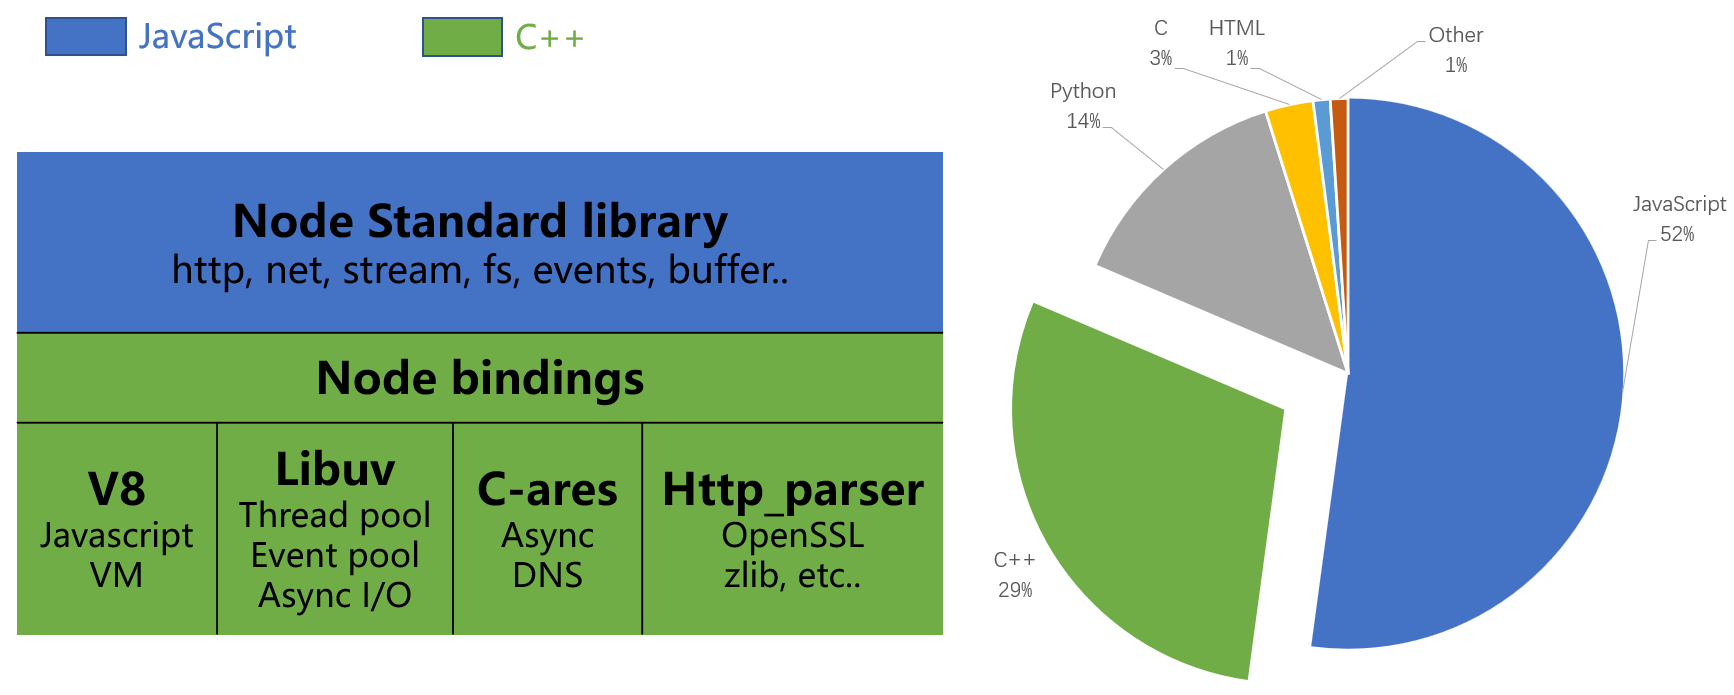
\includegraphics[scale=0.15]{nodecode.png}
\caption{Node.Js源码概览}
\label{fig:label}
\end{figure}
可以看到Node的底层有大量的C++实现,这其中就包括了事件池、系统I/O、线程池等接口的实现,这其实就是标准的服务端底层接口,如对数据库操作的优化、封装,提高查询速度等都是为服务端代码提供,前端只需要提交需要查询的内容,服务端负责读取数据库并返回数据。
当然,说Node是完全服务端的也过于绝对,Node有很强的通用性,就像近年最火的编辑器——VSCode——本来只是一个类似于Atom、Emacs的编辑器,但是有了众多的第三方支持,个人开发者、企业开发者为它制作了成千上万的扩展插件,有良好的生态服务,现在已经可以进行汇编集成开发、
andriod开发等“高端操作”。Node现在有着最大的最活跃的第三方生态社区,甚至有着“能用JS实现的,终将用JS实现”的梗,它已经不再是初始开发时的局限功能。\par
现在,Node对前端开发者应该是最友好的。使用Node,可以构建全自动化脚手架,比如通过Node-gulp,前端开发者可以实现修改完文件之后直接编译、压缩,然后自动刷新浏览器,实时查看修改效果。而且Node采用JS作为编程语言,前端工程师可以直接上手进行服务器编程,实现了前端工程师到
全栈工程师的升级。\par
其实Node也已经无所谓是服务端还是前端了,有了这些丰富的社区支持,Node已经不再只是Node,它已经在曾经不属于它的领域绽放出了光彩。我作为一个小小的JS爱好者,幻想一下,希望能看到“JS实现一切”的那个场景$:)$。

% 这里是简单列表的样例:(如果需要标号自定义或者自动标记数字序号,请自行搜索语法)
% \begin{itemize}
%     \item 简单的列表结构 
%     \item 如这里所示
%     \item 此处仅为样例
%     \item 按需修改和使用
% \end{itemize}


\section{总结}
写本报告大约用了一天的时间,大多时间是在查阅资料、重读PPT,加深自己对计算科学的理解,大部分的总结其实都写在上述文字里。我觉得查阅资料和重读PPT的过程才是收获最多的,读了很多文献、整理了自己的知识链,收获很多。\par
我们应该认识到高校开设的任何一学科都有其滞后性,在我们掌握了一门新技术同时会有更新的技术产生。而我们这一专业更为严重,更为突出,也许在校期间学习的东西在毕业后已经不适合用啦。正如我们现在学习的程序语言,也许在走出校门后又会出现新的语言。所以说,我们要学好这一学科的知识,更需要创新,提高自学能力和接受新事物的能力。我们这一学科本来就是走在时代前沿的一门学科,更需要紧跟时代的步伐。


\newpage
\section{附录}
\begin{itemize}
    \item Github\par
    个人主页
    \url{https://github.com/kngkngtian}\par
    报告仓库
    \url{https://github.com/kngkngtian/Reports}
    \begin{figure}[ht]
        \centering
        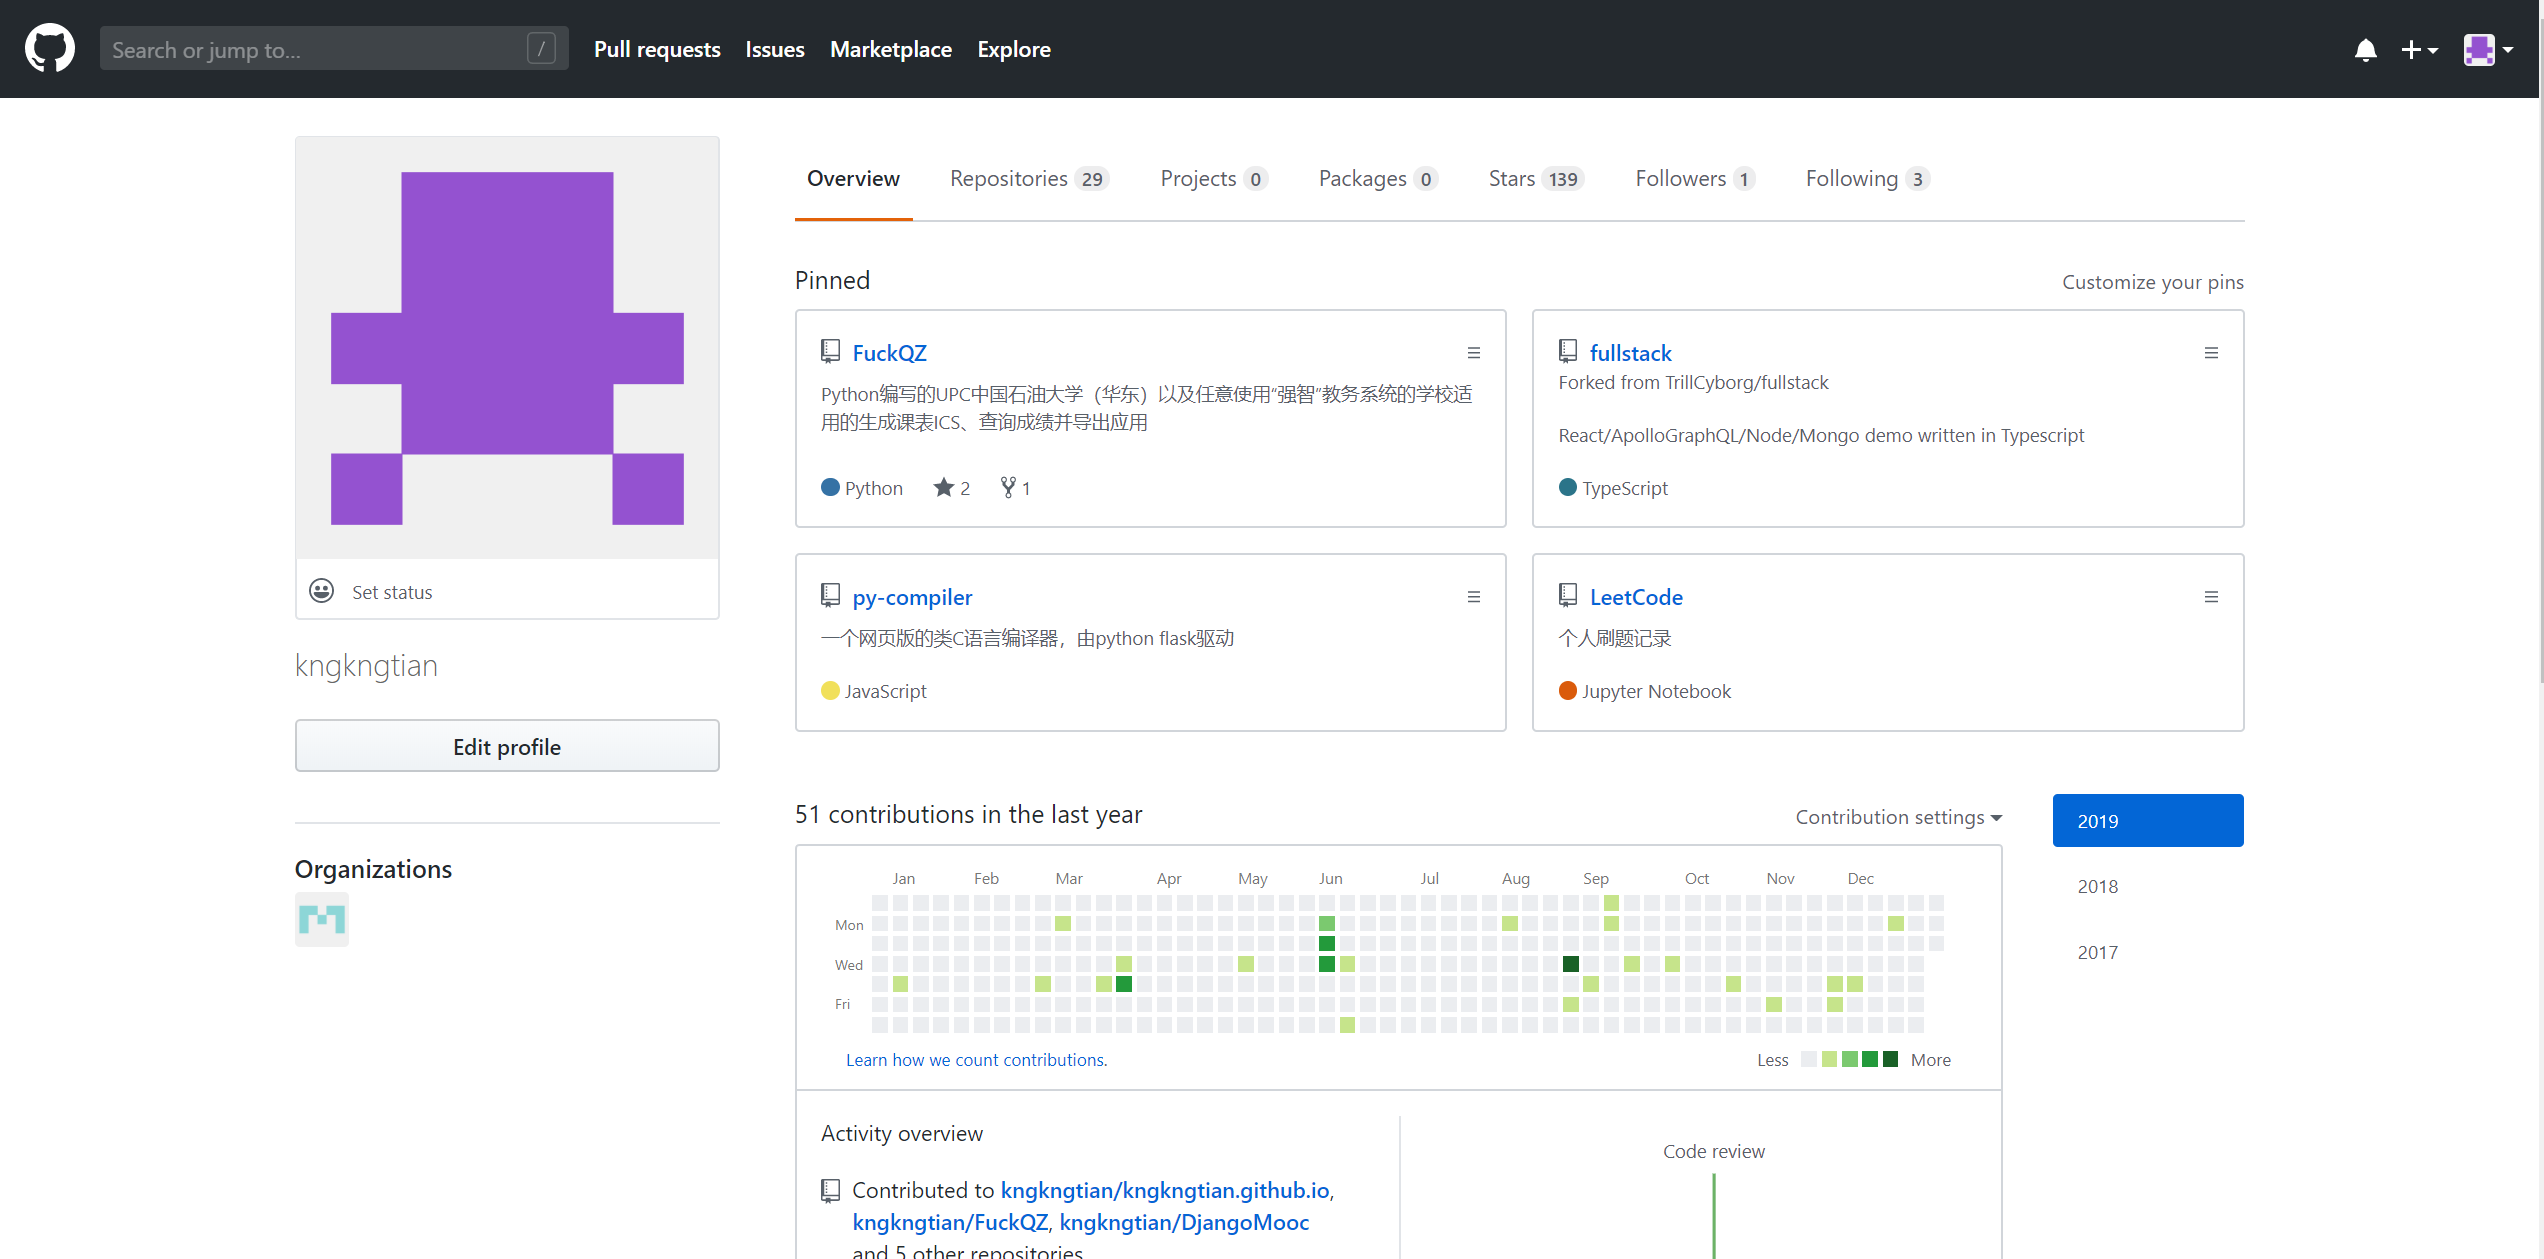
\includegraphics[scale=0.1]{github.png}
        \caption{Github个人主页}
        \label{fig:label}
        \end{figure}
    \newpage
    \item 观察者、学习强国、哔哩哔哩
    \begin{figure}[ht]
        \centering
        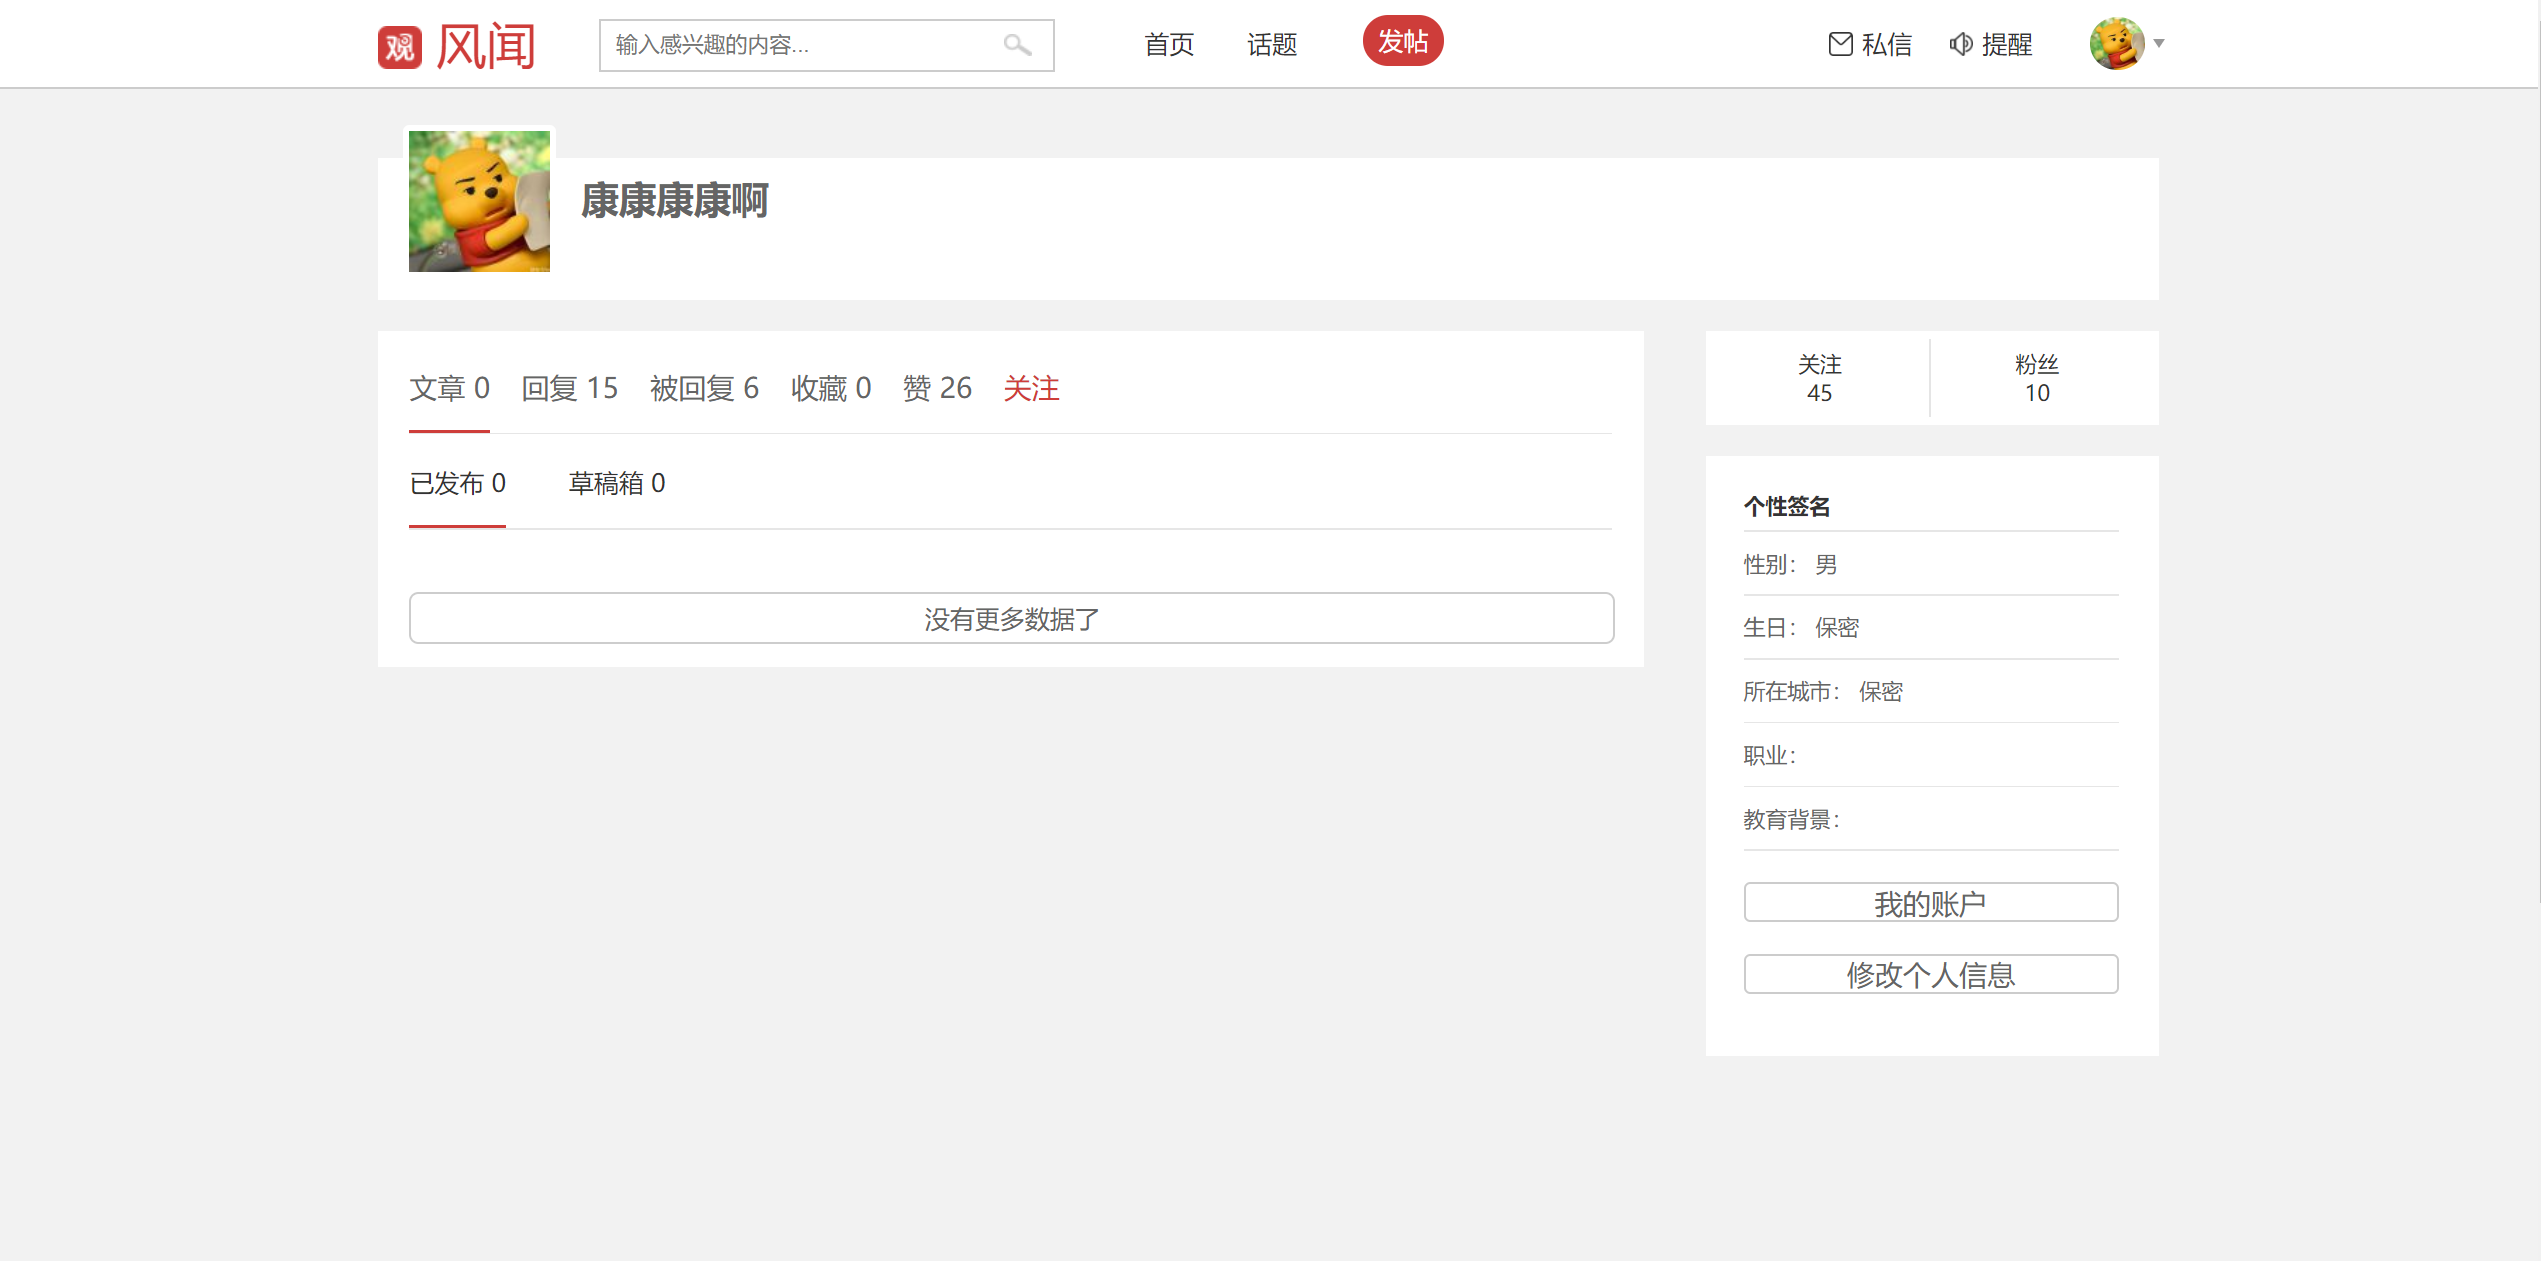
\includegraphics[scale=0.1]{gcz.png}
        \caption{观察者网}
        \label{fig:label}
        \end{figure}
    \begin{figure}[ht]
        \centering
        
\includegraphics[scale=0.11]{xxqg.jpg}
        \caption{学习强国}
        \label{fig:label}
        \end{figure}
    \begin{figure}[ht]
        \centering
        
\includegraphics[scale=0.11]{bilibili.jpg}
        \caption{Bilibili}
        \label{fig:label}
        \end{figure}
    \newpage
    \item CSDN、博客园\par
    CSDN个人主页
    \url{https://blog.csdn.net/coderkang}\par
    \begin{figure}[ht]
        \centering
        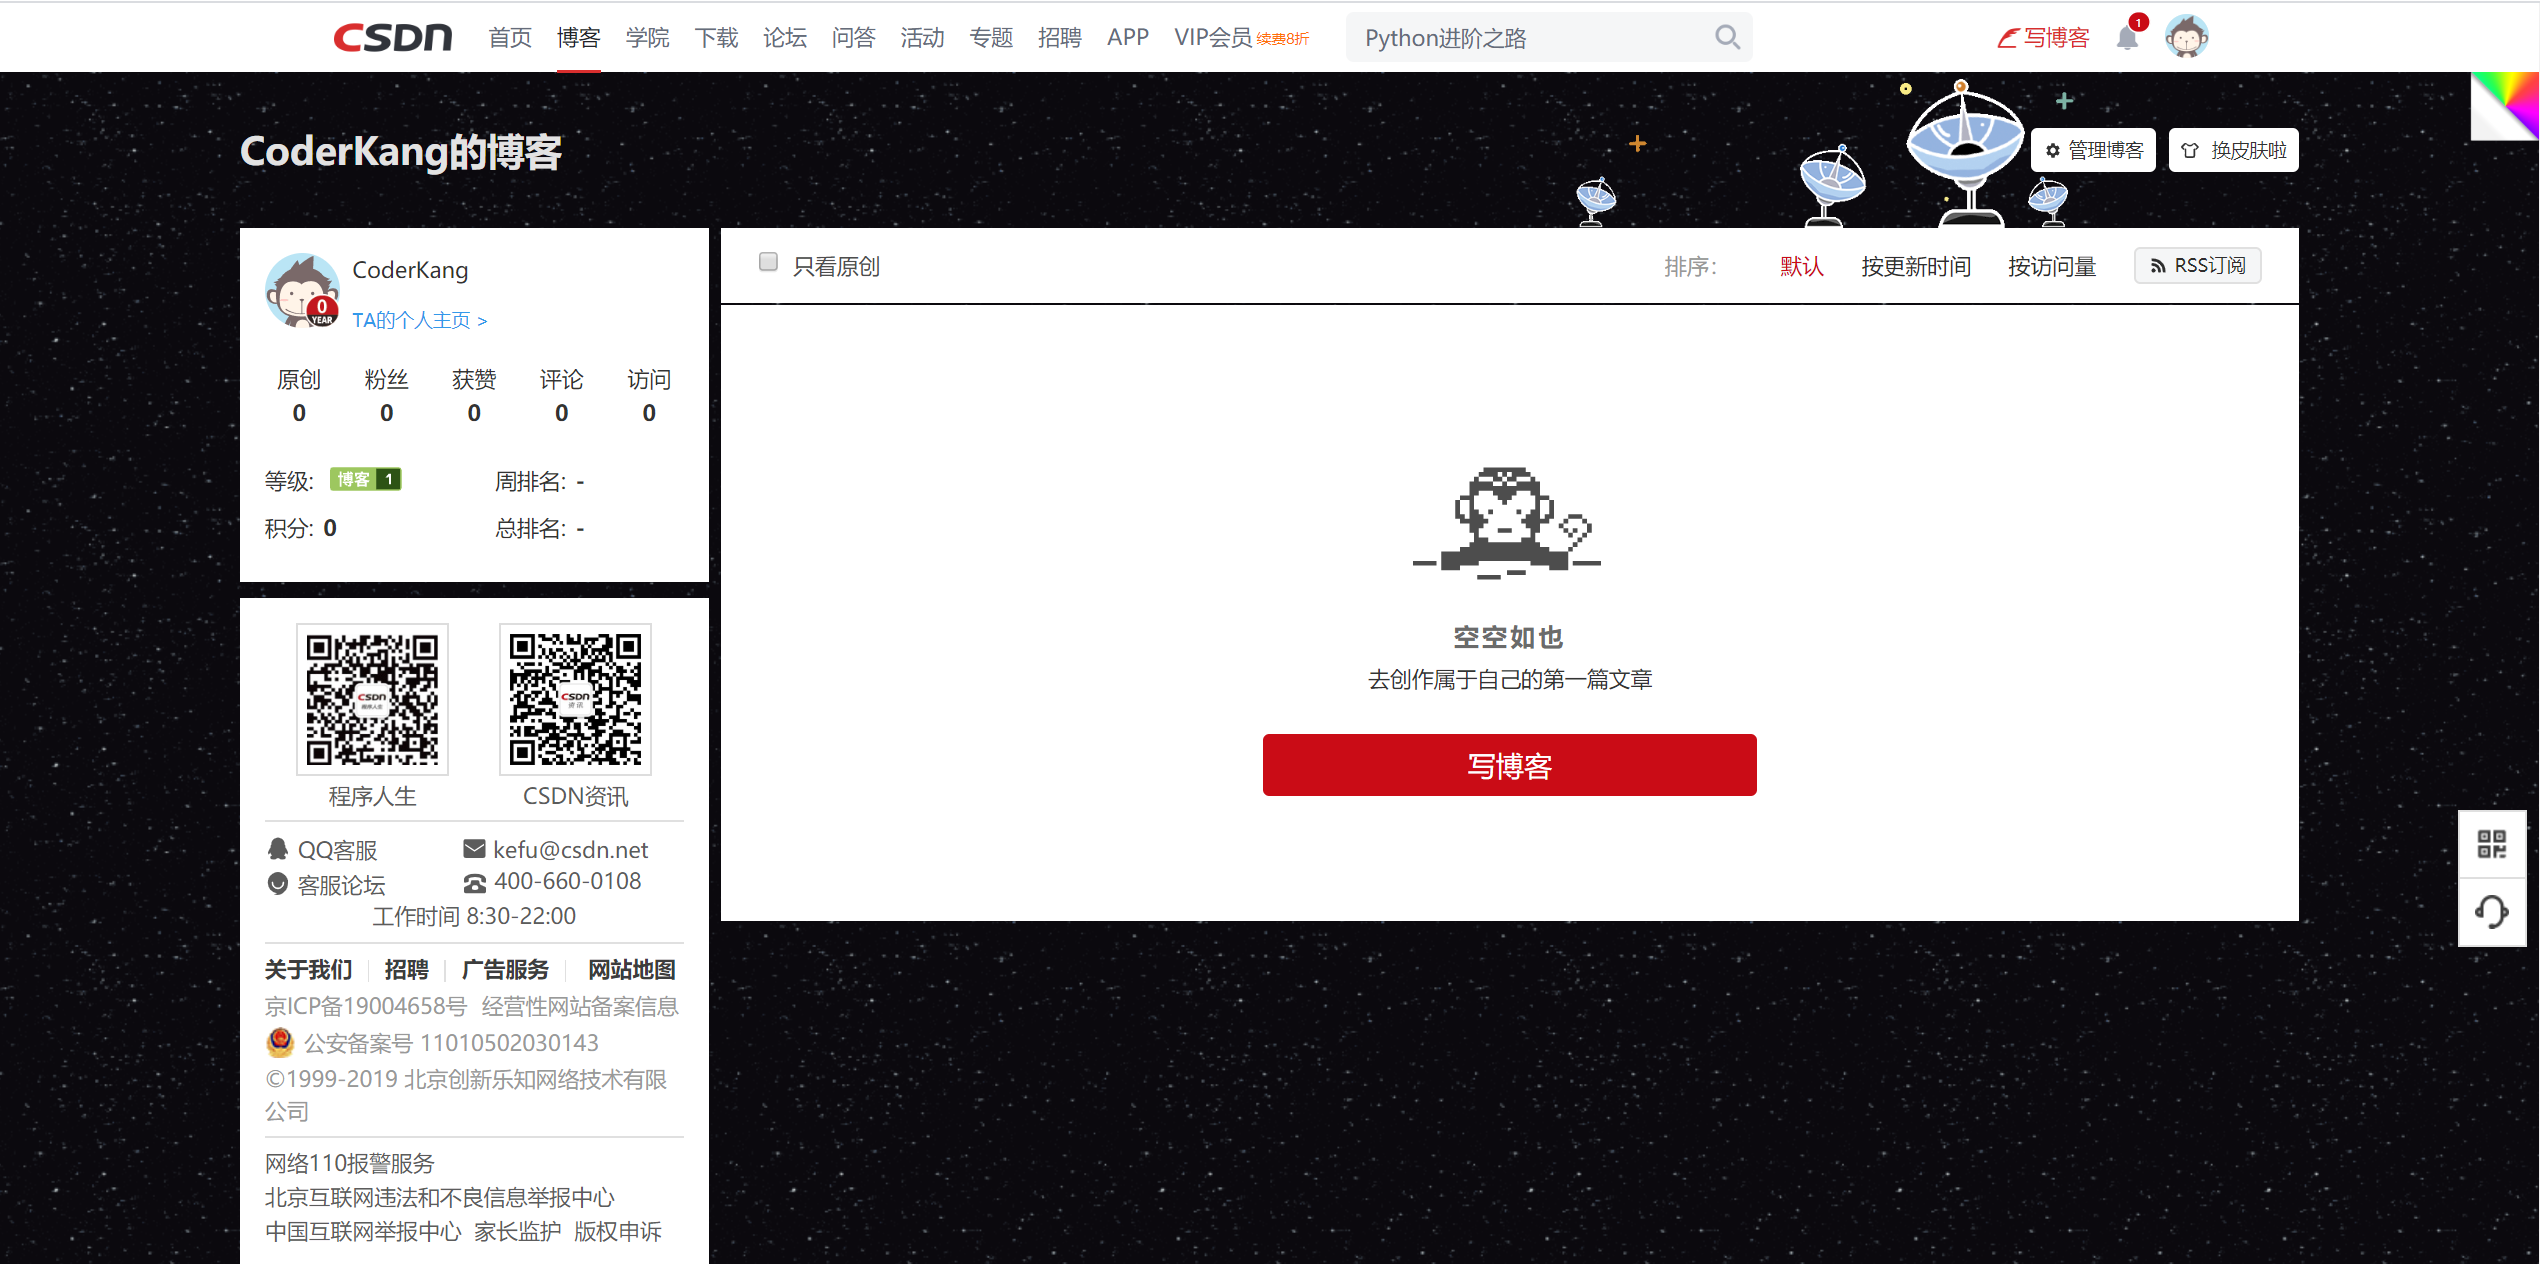
\includegraphics[scale=0.1]{csdn.png}
        \caption{CSDN}
        \label{fig:label}
        \end{figure}
    博客园个人主页
    \url{https://www.cnblogs.com/coderkang/}\par
    \begin{figure}[ht]
        \centering
        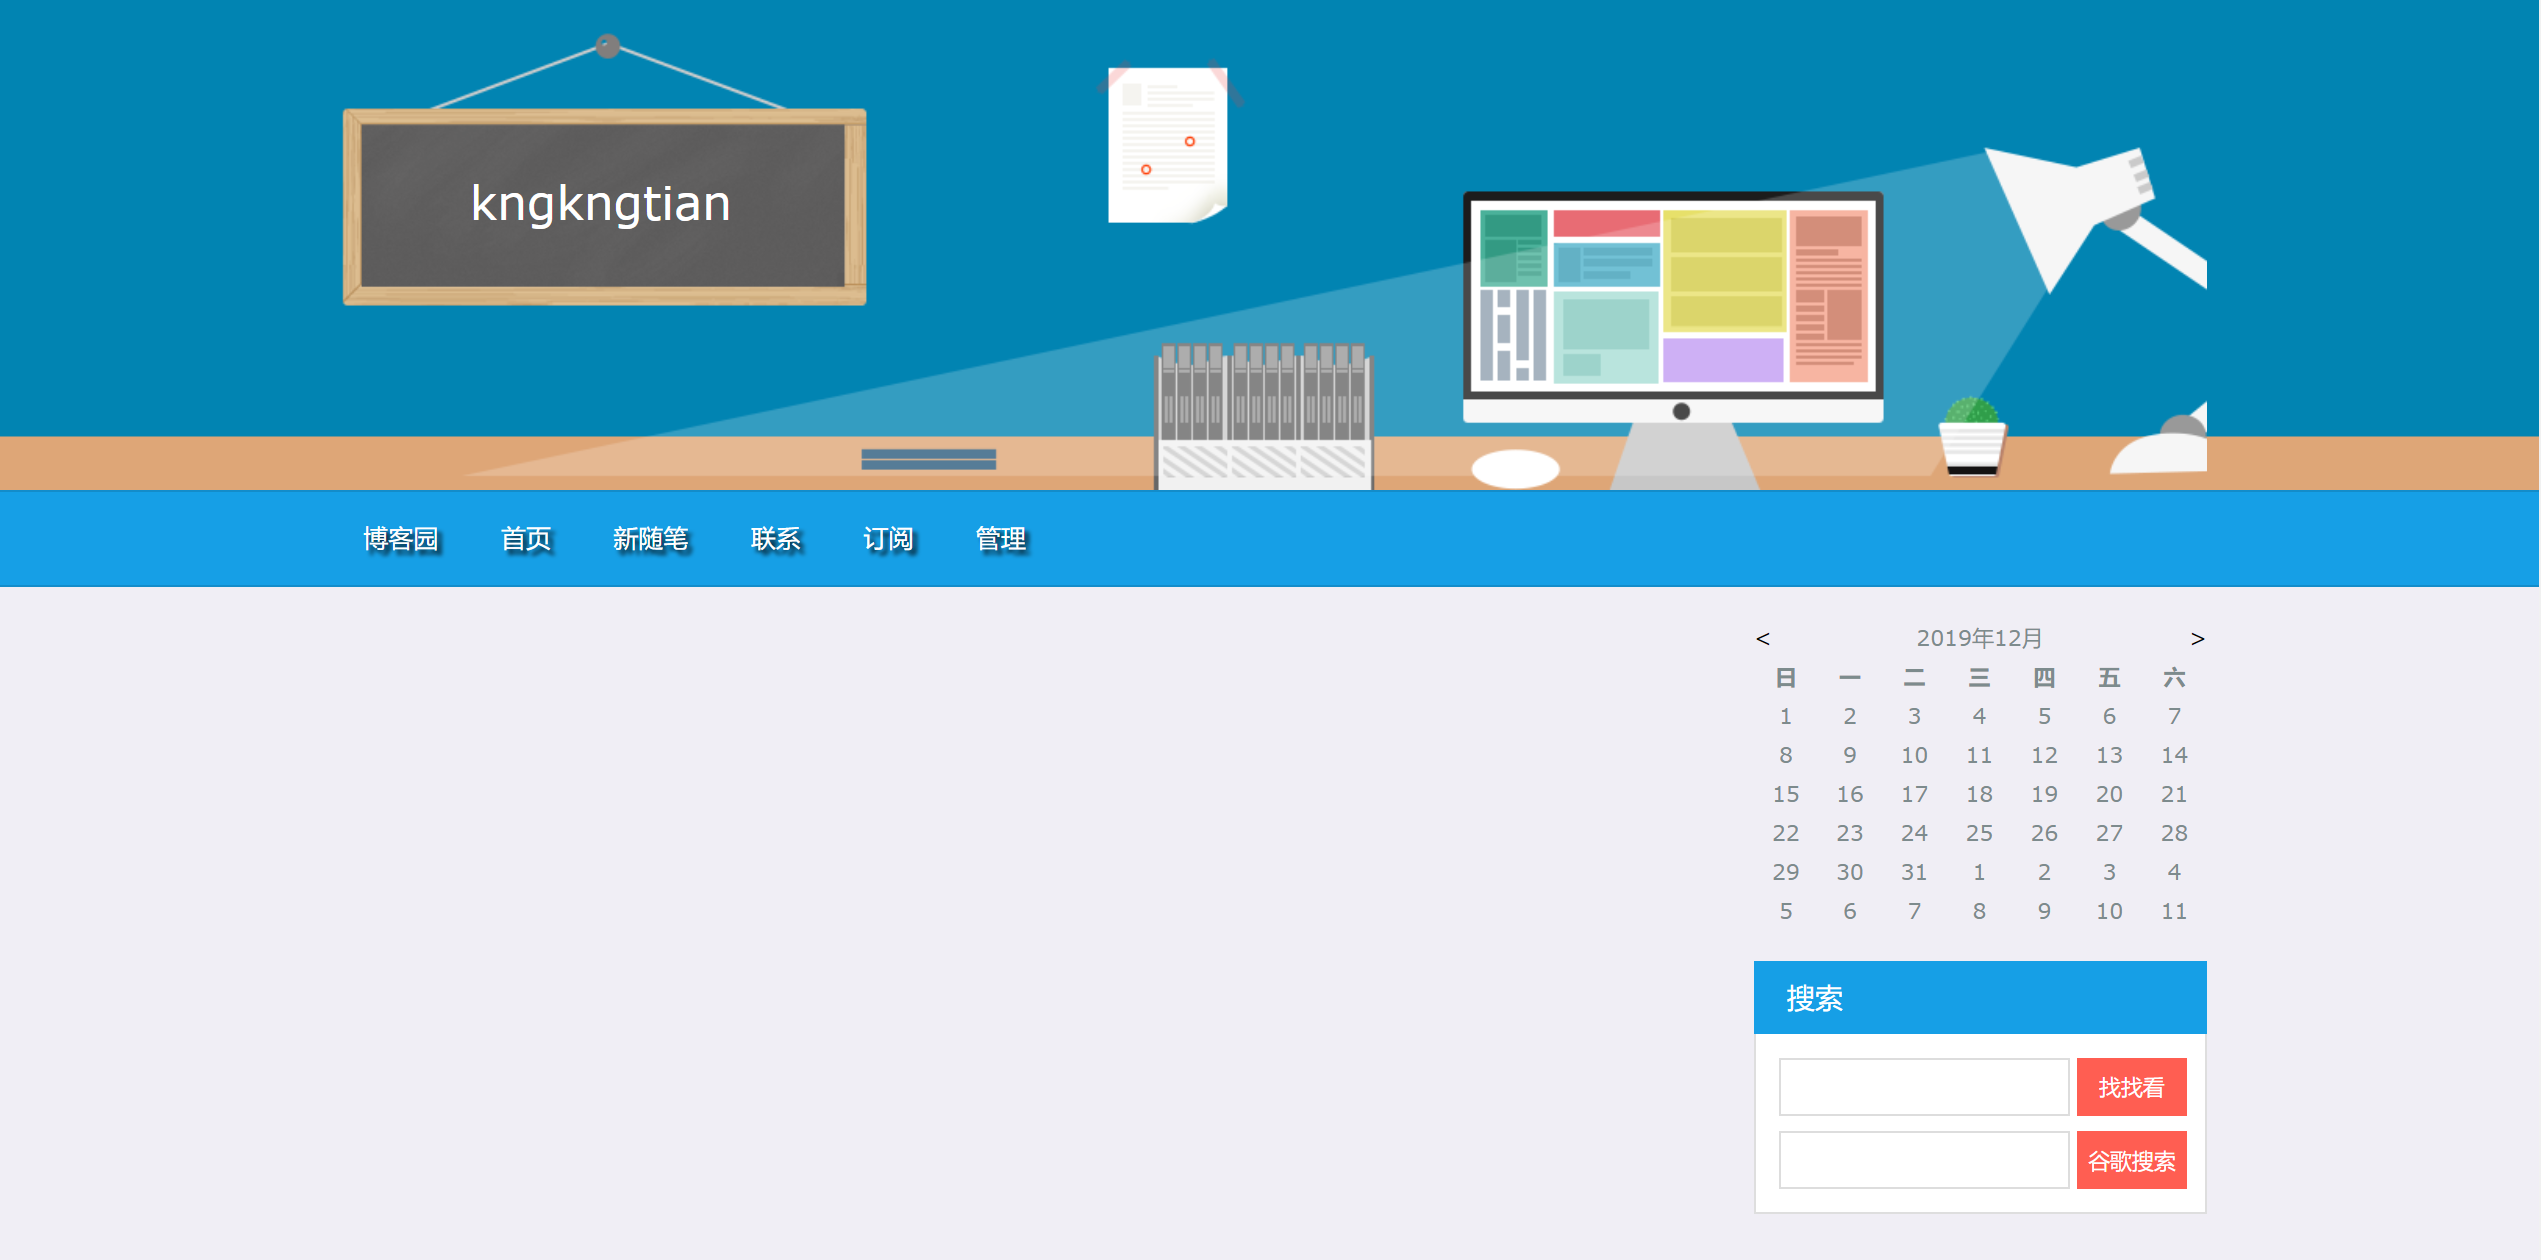
\includegraphics[scale=0.1]{cnblog.png}
        \caption{博客园}
        \label{fig:label}
        \end{figure}
    \item 小木虫\par
    个人网址
    \url{http://muchong.com/bbs/space.php?uid=20339032}\par
    \begin{figure}[ht]
        \centering
        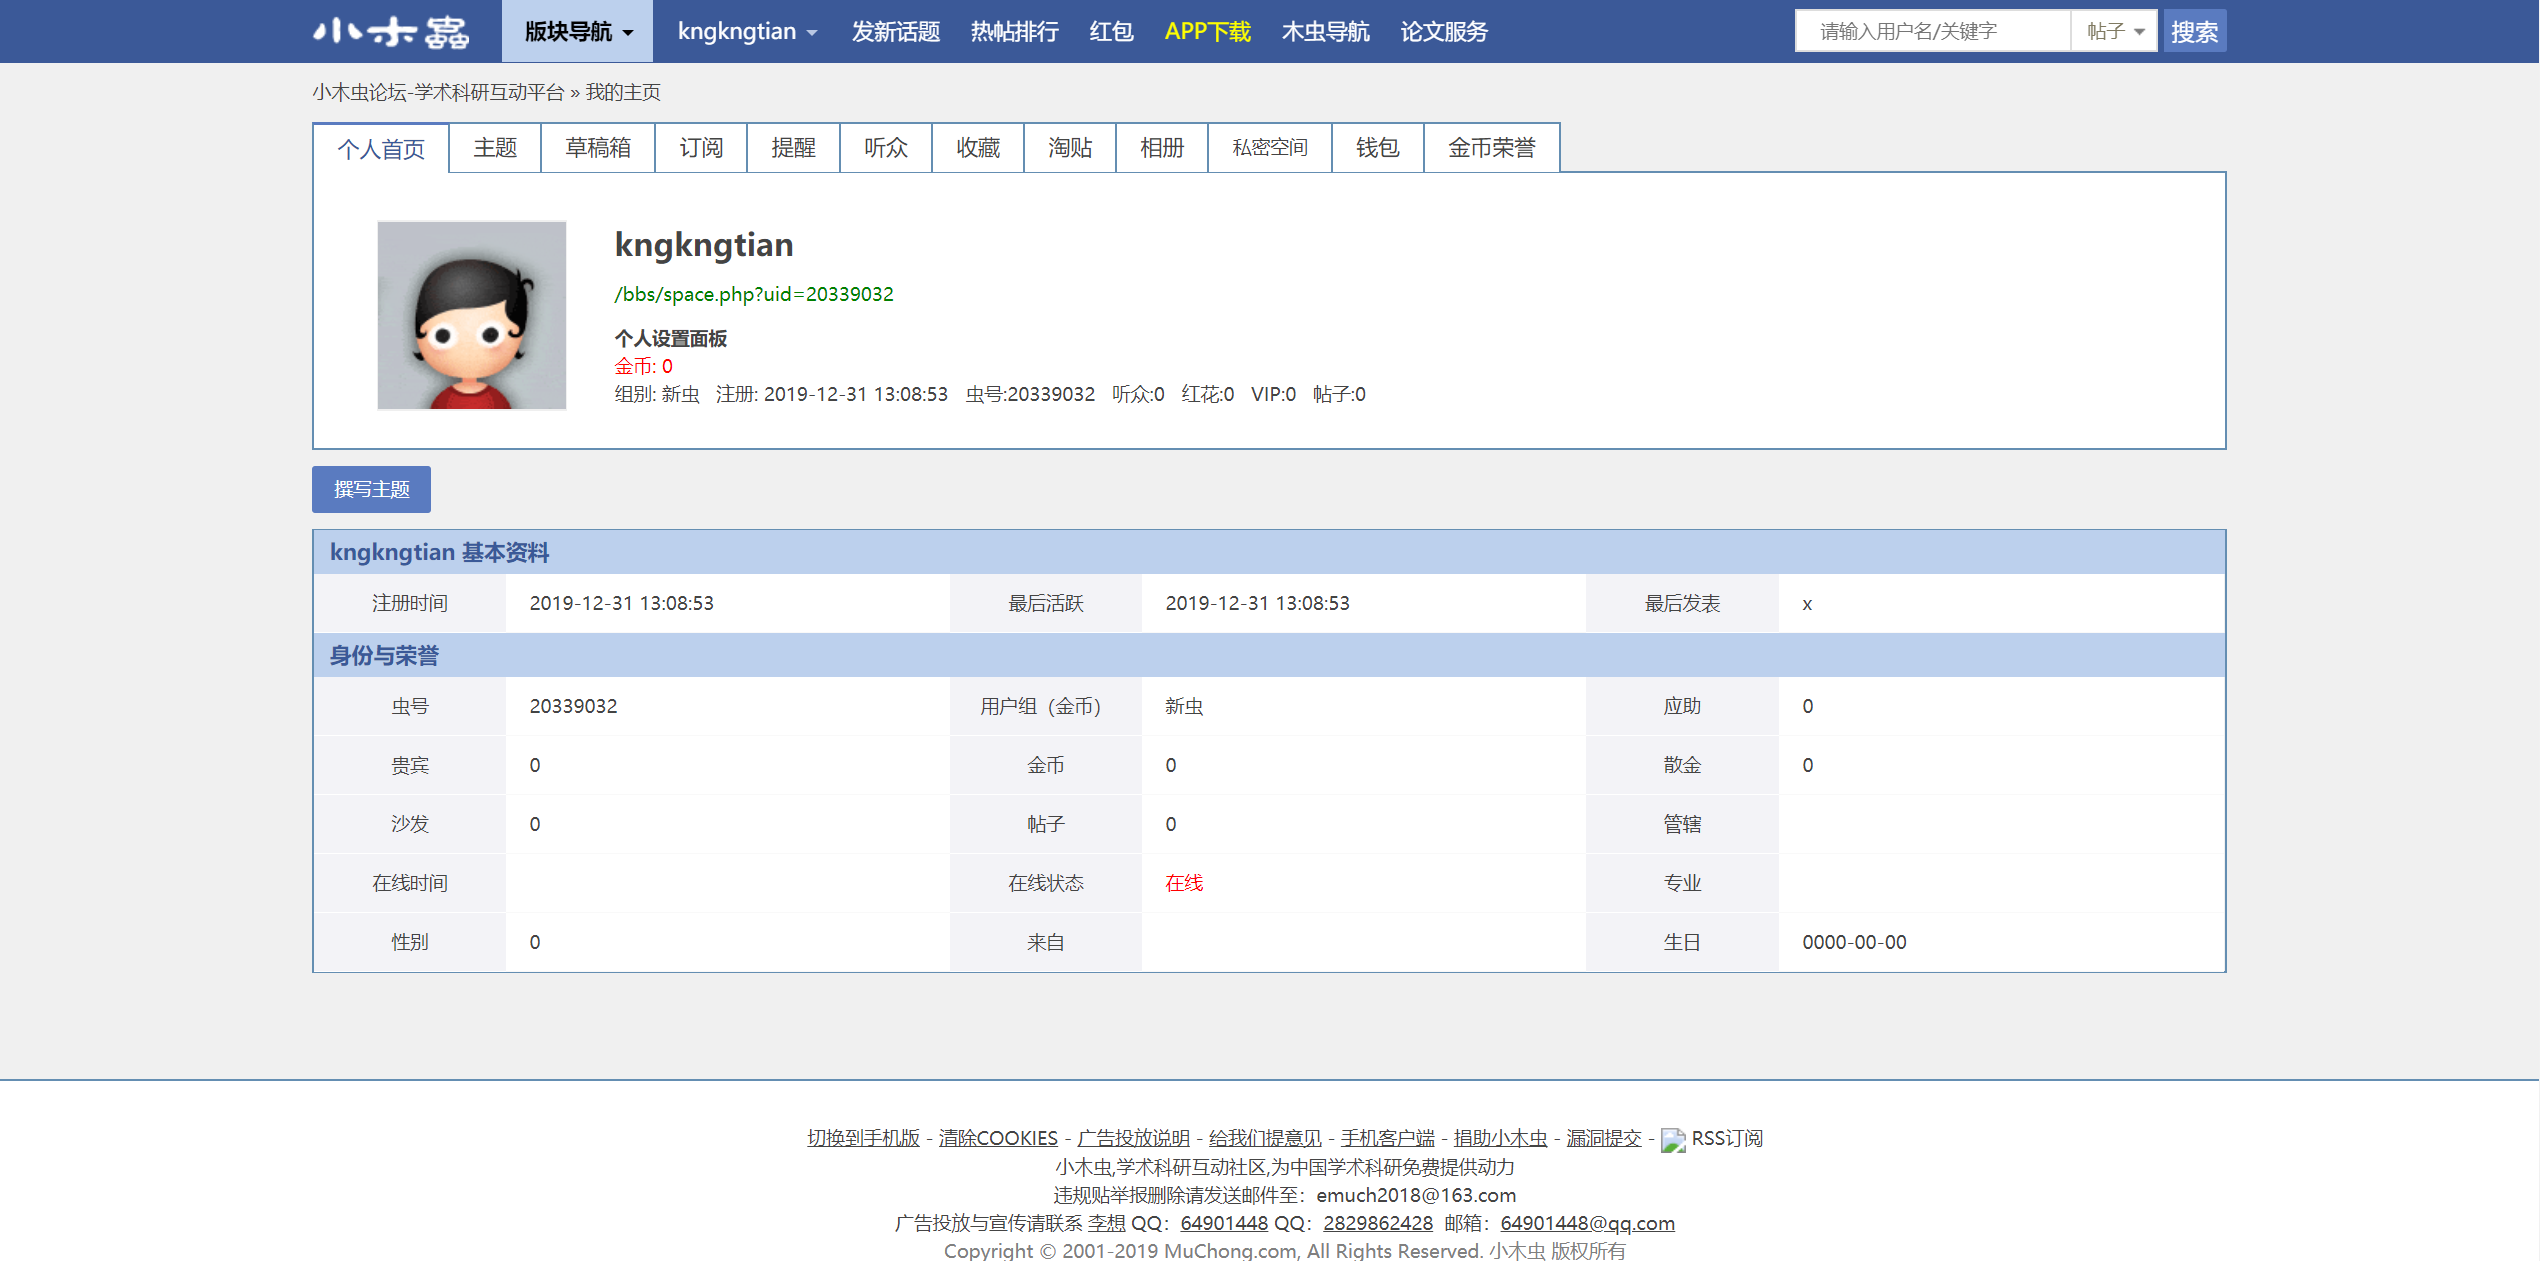
\includegraphics[scale=0.1]{xmc.png}
        \caption{小木虫}
        \label{fig:label}
        \end{figure}
\end{itemize}


\hspace*{\fill} \\

% {\bf 注意,参考文献至少五篇,其中至少两篇为英文文献,参考文献必须在正文中有引用。}
% \bibliographystyle{plain}
\bibliographystyle{unsrt}
\bibliography{references}


\end{document}
